\documentclass{standalone}
\usepackage{graphicx}	
\usepackage{amssymb, amsmath}
\usepackage{color}

\usepackage{tikz}
\usetikzlibrary{intersections, backgrounds}
\usepackage{pgfmath}

\definecolor{light}{RGB}{220, 188, 188}
\definecolor{mid}{RGB}{185, 124, 124}
\definecolor{dark}{RGB}{143, 39, 39}
\definecolor{highlight}{RGB}{180, 31, 180}
\definecolor{gray10}{gray}{0.1}
\definecolor{gray20}{gray}{0.2}
\definecolor{gray30}{gray}{0.3}
\definecolor{gray40}{gray}{0.4}
\definecolor{gray60}{gray}{0.6}
\definecolor{gray70}{gray}{0.7}
\definecolor{gray80}{gray}{0.8}
\definecolor{gray90}{gray}{0.9}
\definecolor{gray95}{gray}{0.95}

\begin{document}

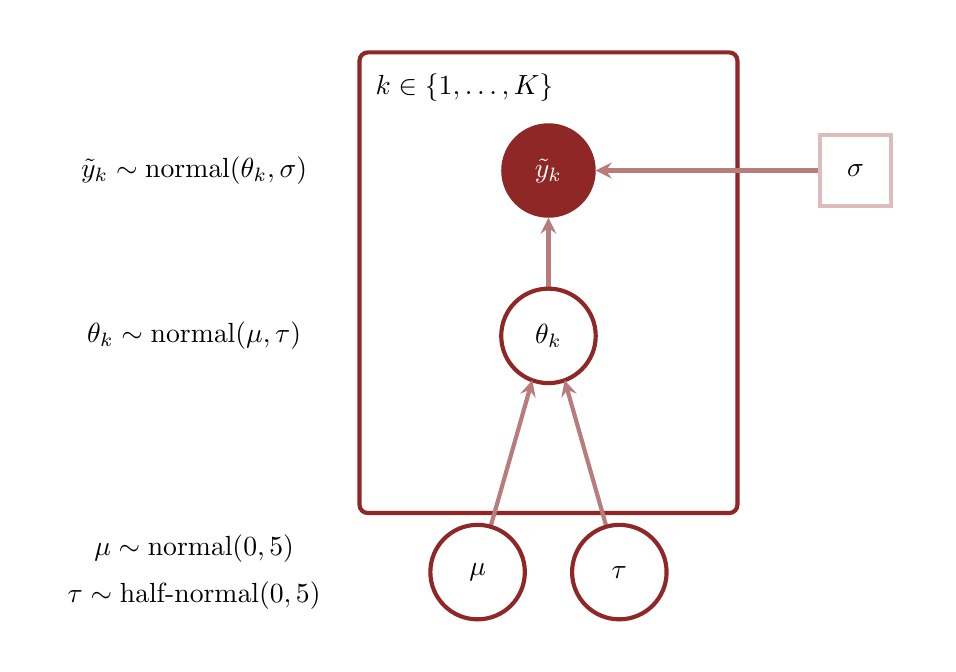
\begin{tikzpicture}[scale=0.3, thick]

\pgfmathsetmacro{\r}{2}

\draw[white] (-22, -13) rectangle (16, 13);

\filldraw[fill=white, draw=dark, line width=1.5, rounded corners=3pt] (-8, -7.5) rectangle (8, 12);

\node[right] at (-7.75, 10.5) { $k \in \{1, \ldots, K \}$ };

\fill[color=dark] (0, 7) circle (\r)
node[color=white] { $\tilde{y}_{k}$ };

\draw[->, >=stealth, color=mid, line width=1.5] (13, 7) -- (0 + \r, 7);

\filldraw[fill=white, draw=light, line width=1.5] (13 - 0.75 * \r, 7 - 0.75 * \r) rectangle +(1.5 * \r, 1.5 * \r);
\node at (13, 7) { $\sigma$ };

\draw[->, >=stealth, color=mid, line width=1.5] (0, 0) -- (0, 7 - \r);

\filldraw[fill=white, draw=dark, line width=1.5] (0, 0) circle (\r)
node[color=black] { $\theta_{k}$ };

\draw[->, >=stealth, color=mid, line width=1.5] (-3, -10) -- ({0 - \r * cos(70)}, {0 - \r * sin(70)});

\filldraw[fill=white, draw=dark, line width=1.5] (-3, -10) circle (\r)
node[color=black] { $\mu$ };

\draw[->, >=stealth, color=mid, line width=1.5] (3, -10) -- ({0 + \r * cos(70)}, {0 - \r * sin(70)});

\filldraw[fill=white, draw=dark, line width=1.5] (3, -10) circle (\r)
node[color=black] { $\tau$ };

\node[] at (-15, 7)    { $\tilde{y}_{k} \sim \text{normal}(\theta_{k}, \sigma)$ };
\node[] at (-15, 0)    { $\theta_{k} \sim \text{normal}(\mu, \tau)$ };
\node[] at (-15, -9)  { $\mu \sim \text{normal}(0, 5)$ };
\node[] at (-15, -11)  { $\tau \sim \text{half-normal}(0, 5)$ };

\end{tikzpicture}

\end{document}  